%------------------------------------------- Sample ------------------------------------

\lipsum[81-100]

\begin{figure}
  \centering
  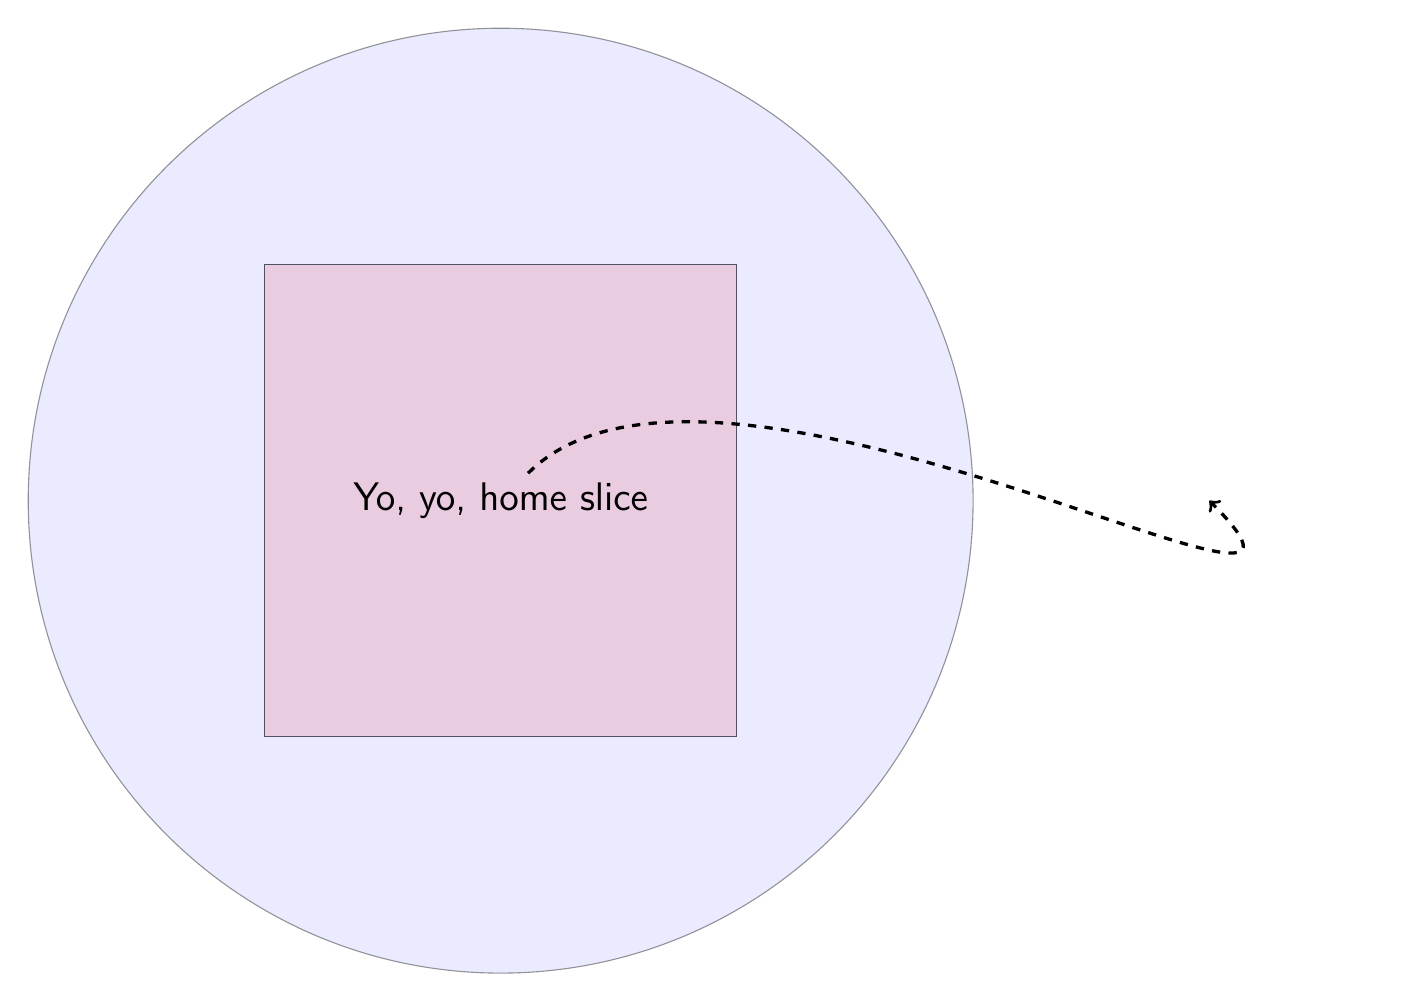
\begin{tikzpicture}[scale=3]

  \draw [fill=red!20!white] (1,1) -- ++(0,-2) -- ++(-2,0) -- ++(0,2) -- cycle;
  \draw [fill=blue!20!white,opacity=0.4] (0,0) circle(2cm);
  \node [font={\Large\sf}] (yo) at (0,0) {Yo, yo, home slice};
  \draw[->,very thick, dashed] (yo) to [out=45,in=-45] (3,0);

\end{tikzpicture}

  \caption[Awesome picture]{Isn't this picture awesome?}
\end{figure}

\begin{figure}
  \centering
  \begin{tikzpicture}
  \draw [fill=red!70!white,circular drop shadow={shadow scale=1.05},very
  thick,rotate=45,opacity=0.7] (0,0) rectangle (3,2);


  \draw [fill=blue!70!white,circular drop shadow={shadow scale=1.05},very
  thick,rotate=135,opacity=0.7] (0,0) rectangle (3,2);
  \draw [fill=orange!70!white,circular drop shadow={shadow scale=1.05},very
  thick,rotate=225,opacity=0.7] (0,0) rectangle (3,2);
  \draw [fill=green!70!white,circular drop shadow={shadow scale=1.05},very
  thick,rotate=-45,opacity=0.7] (0,0) rectangle (3,2);
\end{tikzpicture}

  \caption[Tubular picture]{Totally tubular, dude}
\end{figure}

%------------------------------------------- Real ----------------------------------------

\section{Outer flow}

\subsection{Lagrangian description}

\subsection{Fast vortex methods}
The straightforward method of computing the velocity induced by every particle requires O($N^2$) operations for $N$ vortex elements.
This precludes high-resolution studies of bluff body flows with more than say 50000 elements.
However, fast methods exist that have operation counts of O($N\log N$)  (Barnes \& Hut 1986) or O($N$) (Greengard \& Rocklin 1987) depending on the details of the algorithm.
The basic idea of these methods is to decompose the element population spatially into clusters of particles and build a hierarchy of clusters or a 'tree' - smaller neighboring clusters combine to form a cluster of the next size up in the hierarchy and so on.

The contribution of a cluster of particles to the velocity of a given vortex can then be computed to desired accuracy if the particle is sufficiently far from the cluster in proportion to the size of the cluster and a sufficiently large number of terms in the multipole expansion is taken.
This is the essence of the 'particle-box' method, requiring O($N\log N$) operations.
One then tries to minimize the work required by maximizing the size of the cluster used while keeping the number of terms in the expansion within a reasonable limit and maintaining a certain degree of accuracy.

The 'box-box' scheme goes one step further as accounts for box-box interactions as well. 
These interactions are in the form of shifting the expansions of a certain cluster with the desired accuracy to the center of another cluster.
Then those expansions are used to determine the velocities of the particles in the second cluster.
This has the effect of minimizing the tree traversals for the individual particles, requiring only $O(N)$ operations.
In our numerical implementation, this scheme is utilized.

\section{Inner flow}

\section{Coupling}
